\chapter{Ход работы}
\label{ch:chap2}

\section*{\textbf{Система массового обслуживания}}

Математическая модель, описывающая процессы, в которых объекты (клиенты, заявки, задачи) поступают в систему для обслуживания 
ограниченными ресурсами (каналами обслуживания, операторами, устройствами).

\section*{\textbf{Базовые характеристики}}

$\lambda$ - средняя интенсивность заявок, т.е то кол-во заявок, которое в среднем поступает в СМО в единицу времени, 
$u$ - средняя интенсивность обслуживания, т.е то кол-во заявок, которое в среднем СМО обрабатывает в единицу времени. \\

$t_n$ - набор чисел, каждое чсило указывает на время поступления n-ой заявки в СМО, $v_n$ - интервалы между поступлениями, т.е
разница между $t_{n}$ и $t_{n-1}$. 

\section*{\textbf{Наименования СМО}}

Часто СМО могут называться следующим образом: M/M/1, M/G/1, G/G/2 и т.д. Здесь первый символ - распределение времени между 
поступлениями, второй - распределение времени обслуживания, число в конце - число обслуживающих устройств.

\section*{\textbf{Причем здесь распределения}}

Очень часто хотелось бы иметь возможность прогназировать нагрузку, которая будет приходиться на СМО, чтобы уметь с этой нагрузкой
справляться. Для этого СМО первое время собирает статистические данные о времени поступления заявок и их интесивности. Далее
в этих данных ищутся закономерности, если удается найти закономерность (нашли какой нибудь закон распределения), то можно на будущее
прогнозировать нагрузку. Если закономерности не выявлено (заявки поступают рандомно), то очень часто используют экспоненциальное
распределение.

\section*{\textbf{Пример}}

В магазинах часто много касс, но работают из них в лучшем случае только две. За пару дней до Нового Года,
нагрузка резко возрастает, и в магазинах зачастую начинают работать все кассы. Работники магазинов на основе статистических данных
за прошлые года выявили следующую закономерность: перед Новым Годом большое кол-во покупателей, поэтому они увеличивают кол-во 
устройств обслуживания (касс). Логично, что весь год держать все кассы открытыми экономически невыгодно, т.к большинство
из них будут простаивать, но вместо этого можно отправить кассиров делать работу в зале.

\section*{\textbf{Про сравнение разных СМО}}

Допустим, мы собрали статистические данные и выявили какую-то закономерность, но вопрос в том, является ли распределение, которое
мы вывели самым эффективным? Здесь и нужно сравнение СМО. Чтобы сравнение было корректным, необходимо, чтобы совпадали мат.ожидание
и дисперсия $t_n$ и $v_n$ совпадали. Если они не будут совпадать, то мы начнем сравнивать разные СМО с РАЗНОЙ нагрузкой. Для сравнения
необходимо, чтобы нагрузка была одинаковой, тогда точно можно будет сказать, какая СМО лучше.

\section*{\textbf{Выполнение лабораторной работы}}

Зададим данные для СМО, которая будет иметь экспоненциальное распределение времени поступления заявок. Высчитаем мат.ожидание и дисперсию:

\begin{lstlisting}
    %define params for exp distr

    lambda = 5;
    u = 15;

    %compute E and D for exp distr

    E = 1/lambda;
    D = 1/lambda^2;
\end{lstlisting}

Предположим, что мы хотим сравнить эту СМО с другой СМО, которая имеет хи-квадрат распределение времени поступления заявок. В таком
случае необходимо решить систему из двух уравнений:

\[
\begin{cases}
d = E \\
2d = D
\end{cases}
\]
Такая система не имеет решения, с одной стороны $d = E$, а с другой $d = \frac{D}{2}$. Я взял решение первого уравнения и сложил
с решением второго и поделил пополам (нашел усредненное значение), которое равно 0.11. \\

Теперь зададим 2 выборки: экспоненциальную и хи-квадрат, расчитаем для каждой мат.ожидание и дисперсию:

\begin{lstlisting}
    N = 250;

    chi_seq = chi2rnd(d, N, 1);
    exp_seq = exprnd(E, N, 1);

    chi_E = sum(chi_seq)/N;
    chi_D = sum(chi_seq .^ 2)/N - chi_E^2;

    exp_E = sum(exp_seq)/N;
    exp_D = sum(exp_seq.^2)/N - exp_E^2;
\end{lstlisting}

Сравним показатели:

\begin{lstlisting}
    fprintf("Theory stats: \n");
    fprintf("Exp disrt: E = %f  D = %f\n", E, D);
    fprintf("Chi^2 disrt: E = %f  D = %f\n", d, 2*d);

    fprintf("Real stata: \n");
    fprintf("Exp disrt: E = %f  D = %f\n", exp_E, exp_D);
    fprintf("Chi^2 disrt: E = %f  D = %f\n", chi_E, chi_D);

\end{lstlisting}

Результат:


\begin{figure}[H]
    \centering
    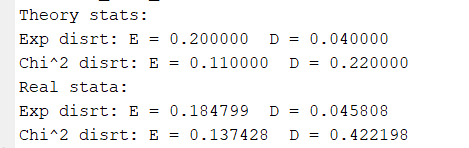
\includegraphics[width=1.0\textwidth]{stats.png}
    \caption{Результаты вычислений}
\end{figure}

Можем заметить, что для каждого распределения статистические мат.ожидание и дисперсия совпадают с теоеретическими с некоторой
допустимой погрешностью. Также можно заметить, что у разных распределений совпадает мат.ожидание (тоже с некоторой
допустимой погрешностью). Как раз это и необходимо для сравнения СМО.

\section*{\textbf{Конртольные вопросы}}

\begin{figure}[H]
    \centering
    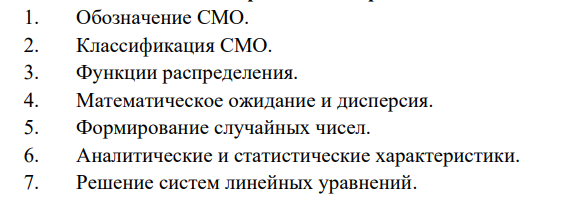
\includegraphics[width=1.0\textwidth]{control.png}
    \caption{Контрольные вопросы}
\end{figure}

\begin{enumerate}

    \item 
        \begin{figure}[H]
        \centering
        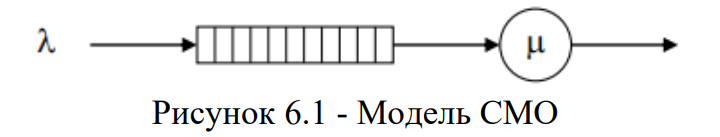
\includegraphics[width=1.0\textwidth]{SMO.png}
        \caption{Обозначение СМО}
        \end{figure}
    \item СМО классифицируются по распределению времени между поступлениями, распределению времени обслуживания, кол-ву обслуживающих устройств.
    \item Способ описаниия случайной величины. Она возвращает вероятность "попасть" в определенный диапазон.
    \item Математическое ожидание - среднее значение, дисперсия - отклонение от мат.ожидания. Могут быть расчитаны теоретически и экспереминтально.
    \item В MATLAB много встроенных функций для генерации выборки из разных распределений (гамма, экспоненциальное, хи-квадрат и т.д).
    \item Аналитическая характеристика - теоретическая, статистическая - полученная на практике.
    \item Для систем решения линейных уравнений применяются методы Гаусса, Крамера, Якоби, Зейделя.
\end{enumerate}

\endinput
